% Figure 3: statistical guarantees (A) and optimization guarantees (B).
% Compile: pdflatex guarantees_map.tex
% Panel B is schematic; its coordinates encode no computed values.
% B-step (solid blue); Omega-step (dashed ochre).
\documentclass[border=9pt]{standalone}
\usepackage[T1]{fontenc}
\renewcommand{\rmdefault}{ptm}
\usepackage{amsmath,amssymb}
\usepackage{fix-cm}
\usepackage{tikz}
\usetikzlibrary{arrows.meta,positioning,calc,backgrounds}
\definecolor{statblue}{RGB}{38,69,109}
\definecolor{optorange}{RGB}{160,91,33}
\definecolor{ink}{RGB}{47,51,56}
\definecolor{muted}{RGB}{96,103,111}
\tikzset{
  resultbox/.style={draw=statblue!75,line width=.55pt,rounded corners=1.5pt,
    fill=statblue!4,align=center,inner xsep=4.5pt,inner ysep=6pt,
    font=\fontsize{9}{10.3}\selectfont,minimum height=1.40cm},
  statarrow/.style={-{Stealth[length=2.0mm,width=1.4mm]},line width=.7pt,statblue},
  lightarrow/.style={-{Stealth[length=1.7mm]},line width=.6pt,muted!70,densely dashed},
  % No background fills: labels are positioned physically clear of the lines.
  arrowtext/.style={font=\fontsize{7.5}{8.5}\selectfont,text=ink,align=center,inner sep=0pt},
  paneltitle/.style={anchor=west,font=\bfseries\fontsize{10.5}{12}\selectfont,text=ink,inner sep=0pt},
  smallnote/.style={font=\fontsize{7.5}{8.5}\selectfont,text=muted,inner sep=0pt},
  bstep/.style={statblue,line width=.85pt,-{Stealth[length=1.6mm,width=1.1mm]}},
  ostep/.style={optorange,line width=.85pt,dash pattern=on 2pt off 1.2pt,
    -{Stealth[length=1.6mm,width=1.1mm]}},
  bshort/.style={statblue,line width=.85pt},
  oshort/.style={optorange,line width=.85pt,dash pattern=on 1.6pt off .8pt},
  start/.style={circle,draw=ink,line width=.65pt,fill=white,inner sep=0pt,
    minimum size=4.7mm,font=\fontsize{7.5}{7.5}\selectfont,text=ink}
}
\begin{document}
\begin{minipage}{14.35cm}
\centering
% ---------------- A: preserve the population/sample structure ----------------
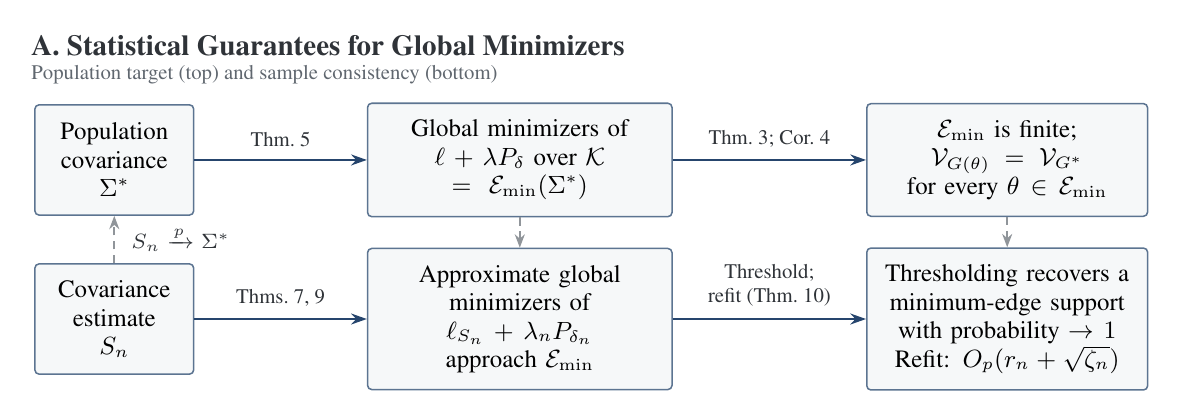
\begin{tikzpicture}[x=1cm,y=1cm]
\path[use as bounding box] (0,.80) rectangle (14.30,5.40);
\node[paneltitle] at (.04,5.17) {A. Statistical Guarantees for Global Minimizers};
\node[smallnote,anchor=west] at (.04,4.80)
  {Population target (top) and sample consistency (bottom)};

\node[resultbox,text width=1.70cm] (pop) at (1.10,3.72)
  {Population\\covariance\\$\Sigma^*$};
\node[resultbox,text width=3.55cm] (target) at (6.25,3.72)
  {Global minimizers of\\$\ell+\lambda P_\delta$ over $\mathcal K$\\$=\mathcal E_{\min}(\Sigma^*)$};
\node[resultbox,text width=3.25cm] (algebra) at (12.44,3.72)
  {$\mathcal E_{\min}$ is finite;\\$\mathcal V_{G(\theta)}=\mathcal V_{G^*}$\\for every $\theta\in\mathcal E_{\min}$};

\node[resultbox,text width=1.70cm] (sample) at (1.10,1.70)
  {Covariance\\estimate\\$S_n$};
\node[resultbox,text width=3.55cm] (approx) at (6.25,1.70)
  {Approximate global minimizers of\\$\ell_{S_n}+\lambda_n P_{\delta_n}$\\approach $\mathcal E_{\min}$};
\node[resultbox,text width=3.25cm] (recover) at (12.44,1.70)
  {Thresholding recovers a\\minimum-edge support\\with probability $\to1$\\Refit: $O_p(r_n+\sqrt{\zeta_n})$};

% Draw all arrows first, then place their labels above or beside them.
\draw[statarrow] (pop.east) -- (target.west);
\draw[statarrow] (target.east) -- (algebra.west);
\draw[statarrow] (sample.east) -- (approx.west);
\draw[statarrow] (approx.east) -- (recover.west);
\node[arrowtext,anchor=south,yshift=4.5pt] at ($(pop.east)!.5!(target.west)$) {Thm.~5};
\node[arrowtext,anchor=south,yshift=4.5pt] at ($(target.east)!.5!(algebra.west)$) {Thm.~3; Cor.~4};
\node[arrowtext,anchor=south,yshift=4.5pt] at ($(sample.east)!.5!(approx.west)$) {Thms.~7, 9};
\node[arrowtext,anchor=south,yshift=4.5pt] at ($(approx.east)!.5!(recover.west)$) {Threshold;\\refit (Thm.~10)};

\draw[lightarrow] (sample.north) -- (pop.south);
\node[arrowtext,anchor=west,xshift=6pt] at ($(sample.north)!.5!(pop.south)$)
  {$S_n\xrightarrow{p}\Sigma^*$};
\draw[lightarrow] (target.south) -- (approx.north);
\draw[lightarrow] (algebra.south) -- (recover.north);
\end{tikzpicture}
\par\vspace{3mm}
% ---------------- B: parameter-space trajectories, not another flowchart ----------------
% All positions below are schematic. No objective values, measured trajectories,
% basin sizes, or convergence-rate estimates are encoded by these coordinates.
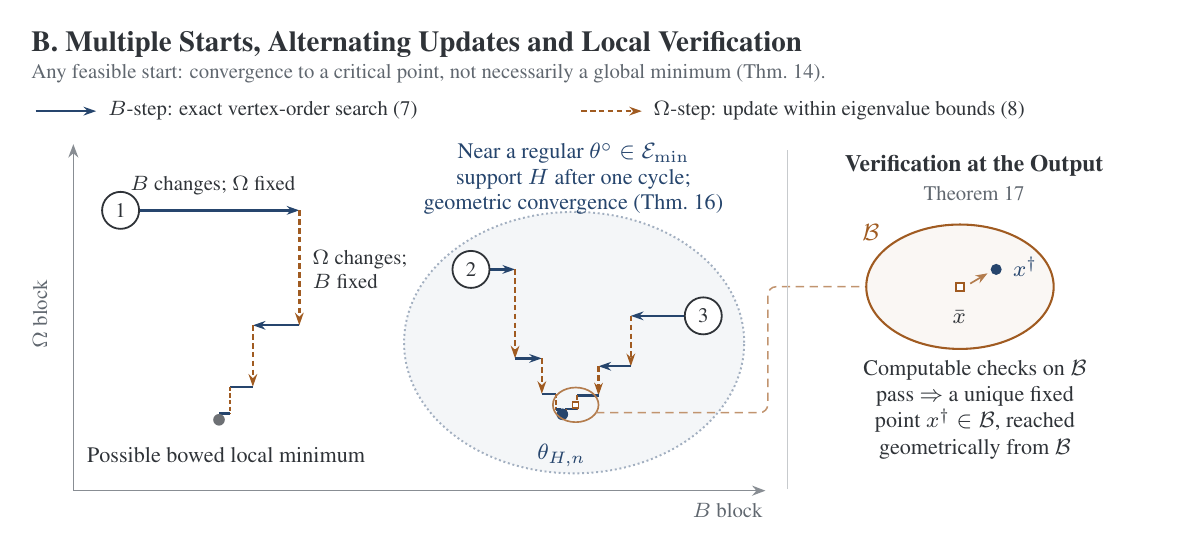
\begin{tikzpicture}[x=1cm,y=1cm]
\path[use as bounding box] (0,.78) rectangle (14.30,7.05);
\node[paneltitle] at (.04,6.84)
  {B. Multiple Starts, Alternating Updates and Local Verification};
\node[smallnote,anchor=west] at (.04,6.46)
  {Any feasible start: convergence to a critical point, not necessarily a global minimum (Thm.~14).};
% Legend: distinguish the two blocks by both color and line pattern.
\draw[bstep] (.10,5.99) -- (.87,5.99);
\node[smallnote,anchor=west,text=ink] at (1.01,5.99)
  {$B$-step: exact vertex-order search (7)};
\draw[ostep] (7.03,5.99) -- (7.80,5.99);
\node[smallnote,anchor=west,text=ink] at (7.94,5.99)
  {$\Omega$-step: update within eigenvalue bounds (8)};

% A two-block parameter-space view. The two axes stand for entire matrix blocks.
\draw[-{Stealth[length=1.7mm]},muted!75,line width=.55pt] (.58,1.17) -- (9.37,1.17);
\draw[-{Stealth[length=1.7mm]},muted!75,line width=.55pt] (.58,1.17) -- (.58,5.57);
\node[smallnote,anchor=north east] at (9.34,1.02) {$B$ block};
\node[smallnote,rotate=90] at (.16,3.41) {$\Omega$ block};

% Local regular neighborhood: no claim that arbitrary starts enter it.
\fill[statblue!5] (6.94,3.05) ellipse [x radius=2.16cm,y radius=1.66cm];
\draw[statblue!43,densely dotted,line width=.7pt]
  (6.94,3.05) ellipse [x radius=2.16cm,y radius=1.66cm];
\node[align=center,font=\fontsize{8}{9.2}\selectfont,text=statblue] at (6.93,5.13)
  {Near a regular $\theta^\circ\in\mathcal E_{\min}$\\
   support $H$ after one cycle;\\geometric convergence (Thm.~16)};

% Run 1: a feasible initialization may reach a non-minimum-edge critical point.
\coordinate (s1) at (1.18,4.73);
\draw[bstep] (s1) -- (3.45,4.73);
\draw[ostep] (3.45,4.73) -- (3.45,3.27);
\draw[bstep] (3.45,3.27) -- (2.86,3.27);
\draw[ostep] (2.86,3.27) -- (2.86,2.49);
\draw[bshort] (2.86,2.49) -- (2.57,2.49);
\draw[oshort] (2.57,2.49) -- (2.57,2.15);
\draw[bshort] (2.57,2.15) -- (2.43,2.15);
\draw[oshort] (2.43,2.15) -- (2.43,2.07);
\node[start] at (s1) {1};
\fill[ink!70] (2.43,2.07) circle (2.1pt);
\node[align=center,font=\fontsize{8}{9.2}\selectfont,text=ink] at (2.52,1.62)
  {Possible bowed local minimum};
\node[smallnote,anchor=south,text=ink] at (2.35,4.92) {$B$ changes; $\Omega$ fixed};
\node[smallnote,anchor=west,text=ink,align=left] at (3.61,3.98)
  {$\Omega$ changes;\\$B$ fixed};

% Runs 2 and 3 start inside the regular neighborhood; both approach theta_H,n.
\coordinate (s2) at (5.63,3.98);
\draw[bstep] (s2) -- (6.19,3.98);
\draw[ostep] (6.19,3.98) -- (6.19,2.85);
\draw[bstep] (6.19,2.85) -- (6.53,2.85);
\draw[ostep] (6.53,2.85) -- (6.53,2.40);
\draw[bshort] (6.53,2.40) -- (6.71,2.40);
\draw[oshort] (6.71,2.40) -- (6.71,2.20);
\draw[bshort] (6.71,2.20) -- (6.77,2.20);
\draw[oshort] (6.77,2.20) -- (6.77,2.14);
\node[start] at (s2) {2};

\coordinate (s3) at (8.58,3.39);
\draw[bstep] (s3) -- (7.66,3.39);
\draw[ostep] (7.66,3.39) -- (7.66,2.75);
\draw[bstep] (7.66,2.75) -- (7.25,2.75);
\draw[ostep] (7.25,2.75) -- (7.25,2.38);
\draw[bshort] (7.25,2.38) -- (6.98,2.38);
\draw[oshort] (6.98,2.38) -- (6.98,2.21);
\draw[bshort] (6.98,2.21) -- (6.83,2.21);
\draw[oshort] (6.83,2.21) -- (6.83,2.15);
\node[start] at (s3) {3};

% The sample fixed point is distinct from the population target theta^circ.
\fill[statblue] (6.79,2.14) circle (2.1pt);
\node[anchor=north,align=center,font=\fontsize{8}{9.2}\selectfont,text=statblue] at (6.78,1.88)
  {$\theta_{H,n}$};
% The computed point is near, not identical to, the fixed point.
\draw[optorange,line width=.65pt,fill=white] (6.92,2.22) rectangle +(0.075,0.075);
\draw[optorange!80,line width=.6pt] (6.96,2.26) ellipse [x radius=.29cm,y radius=.22cm];
% A delicate zoom leader keeps the local certificate visually separate.
\draw[optorange!65,densely dashed,line width=.55pt,rounded corners=3pt]
  (7.22,2.16) -- (9.40,2.16) -- (9.40,3.76) -- (10.65,3.76);

% Verification inset. It is not a statistical or global-optimality certificate.
\draw[muted!35,line width=.4pt] (9.65,1.19) -- (9.65,5.50);
\node[align=center,font=\bfseries\fontsize{8.5}{10}\selectfont,text=ink] at (12.02,5.30)
  {Verification at the Output};
\node[smallnote] at (12.02,4.94) {Theorem~17};
\draw[optorange,fill=optorange!5,line width=.75pt]
  (11.84,3.76) ellipse [x radius=1.19cm,y radius=.79cm];
\node[font=\fontsize{8.5}{10}\selectfont,text=optorange] at (10.71,4.45) {$\mathcal B$};
\draw[optorange,line width=.65pt,fill=white] (11.79,3.71) rectangle (11.89,3.81);
\node[font=\fontsize{8}{9}\selectfont,anchor=north,text=ink] at (11.83,3.58) {$\bar x$};
\fill[statblue] (12.30,3.98) circle (2pt);
\node[font=\fontsize{8}{9}\selectfont,anchor=west,text=statblue] at (12.39,4.01) {$x^\dagger$};
\draw[-{Stealth[length=1.5mm]},optorange!80,line width=.6pt]
  (11.97,3.80) -- (12.19,3.93);
\node[align=center,font=\fontsize{8}{9.5}\selectfont,text=ink] at (12.03,2.20)
  {Computable checks on $\mathcal B$\\
   pass $\Rightarrow$ a unique fixed\\
   point $x^\dagger\in\mathcal B$, reached\\
   geometrically from $\mathcal B$};
\end{tikzpicture}
\end{minipage}
\end{document}
